\subsection{Prime-Time Ratio} \label{subsec:primetime}

The daily diurnal nature of Internet traffic demand requires that ISP providers 
design networks capable of handling load at the times when heaviest usage is 
observed. Such heavy demand is usually observed during prime time hours in the 
evening, when many subscribers heavily consume real-time entertainment traffic
(video) (seen as primarily responsible for high usage during these hours). The FCC defines 
\textbf{Prime-Time} as the local time from 7:00 PM to 11:00 PM.
\cite{fcc2014measuring-broadband}. To measure the concentration of network usage
during prime-time, we use Sandvine's definition of the \textbf{Prime-Time 
ratio}: the ratio of the average traffic demand during prime-time hours to the average 
traffic demand in non-prime-time hours.\cite{sandvine20141h, sandvine20142h}.

We measure the prime-time ratio of the \control{} and \treatment{} group
for each contiguous four hour period in our datasets to find the evening hours with
the largest prime-time ratio. We observed that in our dataset,
the prime time ratio consistently peaks at 8:00 PM -- 12:00 AM for both
datasets.

%\begin{figure}[t]
%\begin{minipage}{1\linewidth}
%\centering
%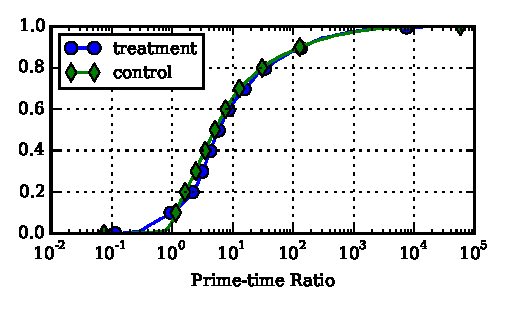
\includegraphics[width=1\linewidth]{figures/prime-time-ratio-per-device-cdf-MEAN.pdf}
%\caption{Prime-Time Ratio\label{fig:cdf-prime-time-ratio}}
%\end{minipage}
%\end{figure}

%\begin{subfigure}[]{.32\linewidth}
%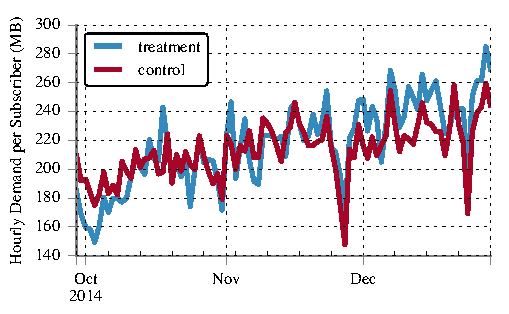
\includegraphics[width=1\linewidth]{figures/primetime_usage_per_day_per_subs.pdf}
%\caption{\label{fig:pt}}
%\end{subfigure}

%\begin{subfigure}[b]{.32\linewidth}
%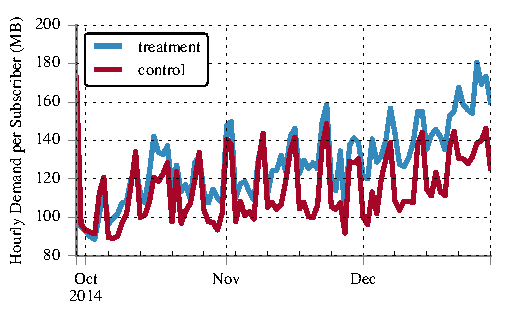
\includegraphics[width=1\linewidth]{figures/nonprimetime_usage_per_day_per_subs.pdf}
%\caption{\label{fig:non-pt}}
%\end{subfigure}


We observed that the hourly downlink traffic per 1000 subscribers between 8:00 PM -- 12:00 AM is 
209.5 GB for \treatment{}, and 205.1 GB for \control{}. However, during an average hour
outside of prime time, the traffic per 1000 subscribers is 122.3 GB for the higher tier
and 108.5 GB for the lower tier. This difference in demand during hours outside of the
daily prime-time is also apparant from the weekly usage patterns in Figure~\ref{fig:traffic-demand-timeseries}.

\begin{table}[t]
\begin{tabular}{| cc | c |c | }\hline
  &                    & Weekday         & Weekends \\\hline
\multirow{2}{*}{\begin{tabular}[c]{@{}l@{}}Hourly Traffic in\\ Prime-Time\end{tabular}}
& treatment          & 233.12          & 246.93   \\
& control            & 225.40          & 238.15   \\\hline
\multirow{2}{*}{\begin{tabular}[c]{@{}l@{}}Hourly Traffic in\\ Non-Prime-Time\end{tabular}}
& treatment & 124.18 & 143.08    \\
& control   & 104.30  & 133.16  \\\hline
\multirow{2}{*}{\begin{tabular}[c]{@{}l@{}}Prime-Time Ratio\end{tabular}}
& treatment & \textbf{1.88} &  1.73 \\
& control  &  \textbf{2.16} &  1.79 \\\hline
\end{tabular}
\caption{Hourly Traffic Demand during in prime-time hours (MB)\label{prime-time-demand}}
\end{table}


We calculate the prime-time ratio per day for the 
datasets groups over weekends and weekdays, as shown in Table \ref{prime-time-demand}.
%in figure~\ref{fig:cdf-prime-time-ratio}. A comparison shows 
On weekends, the prime-time ratios for both groups are
1.73 and 1.79 respectively. On the weekdays, the prime-time ratio for \control{}
is much higher, 2.16, as compared to treatment, 1.88. The demand
during prime-time hours on the weekdays for \treatment{} is within 4\% of
the \control{} traffic, thus there is no substantial
change. In contrast, the demand in non-prime-time hours (outside 8:00 PM -- 12:00 PM)
is much higher in the \treatment{} group, especially on weekdays. 

The average prime-time ratio by traffic volume for the \treatment and \control groups
were 1.70 and 1.93 respectively. However, not all subscribers contribute equally
to the traffic volume. We observed that the median prime-time ratio per subscriber
is 3.39 for the \treatment{} group and 2.91 for the \control{} group. This indicates
that demand during prime-time \emph{per subscriber} has increased, but the total
traffic volume during non-prime-time hours has also increased substantially. For
subscribers that have a larger aggregate demand during non-prime-time hours, the prime
time ratio will be less than one. We found 9\% of the \control{} group and 14\% of 
the treatment group showed this behavior. These subscribers may be small home-run businesses,
users who work at home, or just users who have unexpected usage behaviors.

Initially, we expected that subscribers in the \treatment{} group will increase
their utilization of the link during prime-time hours, when users usually consume video
content. However, overall the \treatment{} group's prime time ratio was 10\% lower than the 
\control{} group. This result indicates that individual subscribers in the higher tier group
have a higher demand than the lower tier during times when the total daily demand is
not within 90\% of its maximum. This extra demand is not enough to bottleneck the service
tier link, yet adds up daily in the total traffic demand per day.


%Latency and performance 
%are adversely affected during prime-time, causing bottlenecks at home, the last 
%mile, in
%transit, or at the content server. For example, the Sandvine Global
%Internet Phenomena Report \footnote{The Sandvine Reports ~\cite{sandvine20141h,
%sandvine20142h}are released bi-annually and
%contain a detailed analysis of aggregate Internet usage. They are also referred
%to in the FCC reports~\cite{fcc2015progress-report, fcc2014measuring-broadband,
%fcc2014progress-report}} showed that devices in the same household selected  
%Netflix's own CDN (OpenConnect) during off-peak hours, and third party CDNs 
%(with differing
%performance) during prime-time. This may happen because Netflix OpenConnect is
%over-utilized during prime time~\cite{sandvine20141h}.